% Slides for 2024-10-07
% To create a slide, use the following:
% \begin{frame}{TITLE}
%     BODY
% \end{frame}

% To create a slide with a bullet list, use the following:
% \begin{frame}{TITLE}
%     \begin{itemize}
%         \item ITEM 1
%         \item ITEM 2
%     \end{itemize}    
% \end{frame}

% To create a slide with numbered list, use the following:
% \begin{frame}{TITLE}
%     \begin{enumerate}
%         \item ITEM 1
%         \item ITEM 2
%     \end{enumerate}
% \end{frame}

% To create a slide with a graphic:
% 1. Add the graphic to this folder (named picture.png)
% 2. Use the following:
% \begin{frame}{TITLE}
%     \centering
%     \includegraphics[height=0.7\textheight,width=0.7\textwidth,keepaspectratio]{picture.png}
% \end{frame}

% To create a slide with two columns, use the following:
% \begin{frame}{TITLE}
%     \begin{columns}
%         \begin{column}{0.5\textwidth}
%             COLUMN 1 BODY
%         \end{column}
%         \begin{column}{0.5\textwidth}
%             COLUMN 2 BODY
%         \end{column}
%     \end{columns}
% \end{frame}

\begin{frame}{Instances are Running}
    \begin{columns}
        \begin{column}{0.6\textwidth}
            \centering
            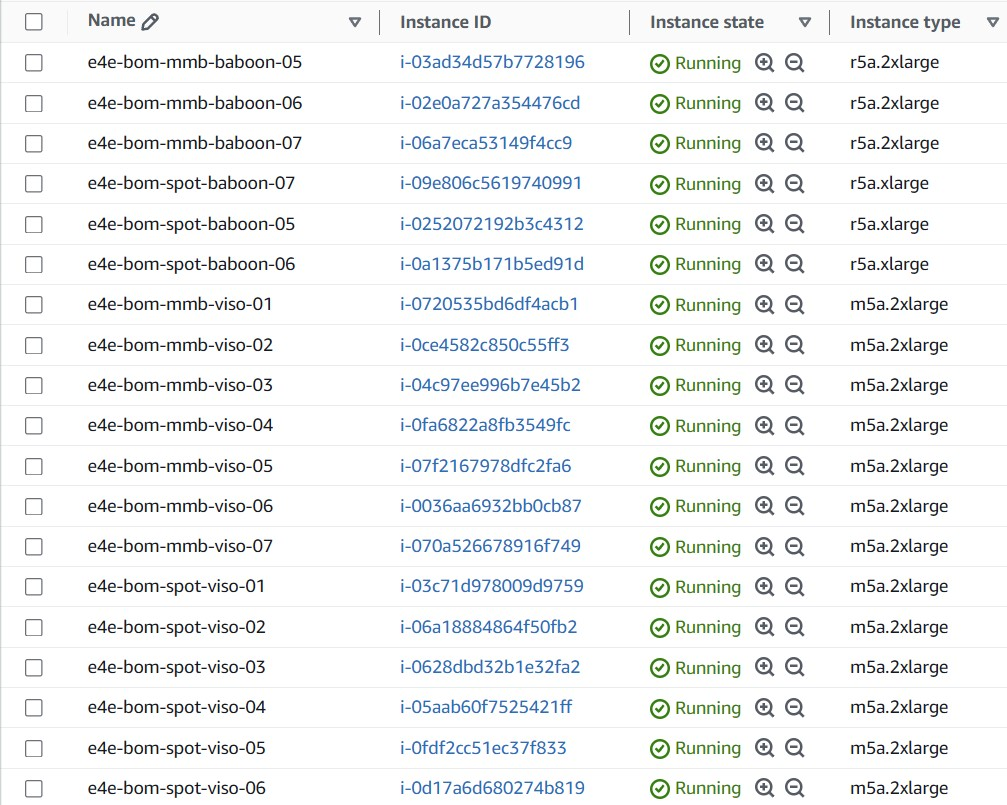
\includegraphics[height=0.8\textheight,width=0.95\textwidth,keepaspectratio]{images/bom/aws.jpg}
        \end{column}
        \begin{column}{0.4\textwidth}
            \begin{itemize}
                \item "It costs 2 cents to run these instances, for 12 seconds."
                \item (\$5000.50 per month)
            \end{itemize}
        \end{column}
    \end{columns}
\end{frame}

\begin{frame}{Paper Questions}
    \begin{itemize}
        \item Is 7 VISO and 3 Baboon enough?
        \begin{itemize}
            \item If yes, probably don't need more money.
        \end{itemize}
        \item Publish dataset?
        \begin{itemize}
            \item First 10s of 7 videos labeled.
            \item Around 20 vidoes from 2-10mins. 
        \end{itemize}
    \end{itemize}
\end{frame}
